\documentclass[twoside]{book}

% Packages required by doxygen
\usepackage{fixltx2e}
\usepackage{calc}
\usepackage{doxygen}
\usepackage[export]{adjustbox} % also loads graphicx
\usepackage{graphicx}
\usepackage[utf8]{inputenc}
\usepackage{makeidx}
\usepackage{multicol}
\usepackage{multirow}
\PassOptionsToPackage{warn}{textcomp}
\usepackage{textcomp}
\usepackage[nointegrals]{wasysym}
\usepackage[table]{xcolor}

% Font selection
\usepackage[T1]{fontenc}
\usepackage[scaled=.90]{helvet}
\usepackage{courier}
\usepackage{amssymb}
\usepackage{sectsty}
\renewcommand{\familydefault}{\sfdefault}
\allsectionsfont{%
  \fontseries{bc}\selectfont%
  \color{darkgray}%
}
\renewcommand{\DoxyLabelFont}{%
  \fontseries{bc}\selectfont%
  \color{darkgray}%
}
\newcommand{\+}{\discretionary{\mbox{\scriptsize$\hookleftarrow$}}{}{}}

% Page & text layout
\usepackage{geometry}
\geometry{%
  a4paper,%
  top=2.5cm,%
  bottom=2.5cm,%
  left=2.5cm,%
  right=2.5cm%
}
\tolerance=750
\hfuzz=15pt
\hbadness=750
\setlength{\emergencystretch}{15pt}
\setlength{\parindent}{0cm}
\setlength{\parskip}{3ex plus 2ex minus 2ex}
\makeatletter
\renewcommand{\paragraph}{%
  \@startsection{paragraph}{4}{0ex}{-1.0ex}{1.0ex}{%
    \normalfont\normalsize\bfseries\SS@parafont%
  }%
}
\renewcommand{\subparagraph}{%
  \@startsection{subparagraph}{5}{0ex}{-1.0ex}{1.0ex}{%
    \normalfont\normalsize\bfseries\SS@subparafont%
  }%
}
\makeatother

% Headers & footers
\usepackage{fancyhdr}
\pagestyle{fancyplain}
\fancyhead[LE]{\fancyplain{}{\bfseries\thepage}}
\fancyhead[CE]{\fancyplain{}{}}
\fancyhead[RE]{\fancyplain{}{\bfseries\leftmark}}
\fancyhead[LO]{\fancyplain{}{\bfseries\rightmark}}
\fancyhead[CO]{\fancyplain{}{}}
\fancyhead[RO]{\fancyplain{}{\bfseries\thepage}}
\fancyfoot[LE]{\fancyplain{}{}}
\fancyfoot[CE]{\fancyplain{}{}}
\fancyfoot[RE]{\fancyplain{}{\bfseries\scriptsize Generated by Doxygen }}
\fancyfoot[LO]{\fancyplain{}{\bfseries\scriptsize Generated by Doxygen }}
\fancyfoot[CO]{\fancyplain{}{}}
\fancyfoot[RO]{\fancyplain{}{}}
\renewcommand{\footrulewidth}{0.4pt}
\renewcommand{\chaptermark}[1]{%
  \markboth{#1}{}%
}
\renewcommand{\sectionmark}[1]{%
  \markright{\thesection\ #1}%
}

% Indices & bibliography
\usepackage{natbib}
\usepackage[titles]{tocloft}
\setcounter{tocdepth}{3}
\setcounter{secnumdepth}{5}
\makeindex

% Hyperlinks (required, but should be loaded last)
\usepackage{ifpdf}
\ifpdf
  \usepackage[pdftex,pagebackref=true]{hyperref}
\else
  \usepackage[ps2pdf,pagebackref=true]{hyperref}
\fi
\hypersetup{%
  colorlinks=true,%
  linkcolor=blue,%
  citecolor=blue,%
  unicode%
}

% Custom commands
\newcommand{\clearemptydoublepage}{%
  \newpage{\pagestyle{empty}\cleardoublepage}%
}

\usepackage{caption}
\captionsetup{labelsep=space,justification=centering,font={bf},singlelinecheck=off,skip=4pt,position=top}

%===== C O N T E N T S =====

\begin{document}

% Titlepage & ToC
\hypersetup{pageanchor=false,
             bookmarksnumbered=true,
             pdfencoding=unicode
            }
\pagenumbering{roman}
\begin{titlepage}
\vspace*{7cm}
\begin{center}%
{\Large My Project }\\
\vspace*{1cm}
{\large Generated by Doxygen 1.8.11}\\
\end{center}
\end{titlepage}
\clearemptydoublepage
\tableofcontents
\clearemptydoublepage
\pagenumbering{arabic}
\hypersetup{pageanchor=true}

%--- Begin generated contents ---
\chapter{File Index}
\section{File List}
Here is a list of all files with brief descriptions\+:\begin{DoxyCompactList}
\item\contentsline{section}{\hyperlink{Lab1_8c}{Lab1.\+c} }{\pageref{Lab1_8c}}{}
\end{DoxyCompactList}

\chapter{File Documentation}
\hypertarget{Solovay-Strassen_8cpp}{}\section{Solovay-\/\+Strassen.cpp File Reference}
\label{Solovay-Strassen_8cpp}\index{Solovay-\/\+Strassen.\+cpp@{Solovay-\/\+Strassen.\+cpp}}
{\ttfamily \#include $<$cstring$>$}\\*
{\ttfamily \#include $<$iostream$>$}\\*
{\ttfamily \#include $<$cstdlib$>$}\\*
Include dependency graph for Solovay-\/\+Strassen.cpp\+:
\nopagebreak
\begin{figure}[H]
\begin{center}
\leavevmode
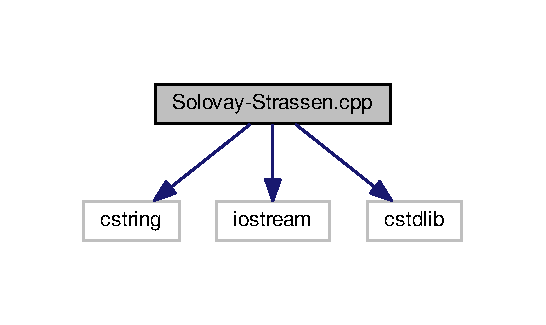
\includegraphics[width=262pt]{Solovay-Strassen_8cpp__incl}
\end{center}
\end{figure}
\subsection*{Macros}
\begin{DoxyCompactItemize}
\item 
\#define \hyperlink{Solovay-Strassen_8cpp_ae1d1ec9482079231e898236e2b23c9ba}{ll}~long long
\end{DoxyCompactItemize}
\subsection*{Functions}
\begin{DoxyCompactItemize}
\item 
\hyperlink{Solovay-Strassen_8cpp_ae1d1ec9482079231e898236e2b23c9ba}{ll} \hyperlink{Solovay-Strassen_8cpp_ad815f4d0c344576558f86d0dd549e7f2}{modulo} (\hyperlink{Solovay-Strassen_8cpp_ae1d1ec9482079231e898236e2b23c9ba}{ll} base, \hyperlink{Solovay-Strassen_8cpp_ae1d1ec9482079231e898236e2b23c9ba}{ll} exponent, \hyperlink{Solovay-Strassen_8cpp_ae1d1ec9482079231e898236e2b23c9ba}{ll} mod)
\item 
int \hyperlink{Solovay-Strassen_8cpp_a8cdb5b6678d3f321ad91e68058ac6306}{calculate\+Jacobian} (\hyperlink{Solovay-Strassen_8cpp_ae1d1ec9482079231e898236e2b23c9ba}{ll} a, \hyperlink{Solovay-Strassen_8cpp_ae1d1ec9482079231e898236e2b23c9ba}{ll} n)
\item 
bool \hyperlink{Solovay-Strassen_8cpp_a65b69102e0221bb5cfcb7485dffda0d0}{Solovoy} (\hyperlink{Solovay-Strassen_8cpp_ae1d1ec9482079231e898236e2b23c9ba}{ll} p, int iteration)
\item 
int \hyperlink{Solovay-Strassen_8cpp_ae66f6b31b5ad750f1fe042a706a4e3d4}{main} ()
\end{DoxyCompactItemize}


\subsection{Macro Definition Documentation}
\index{Solovay-\/\+Strassen.\+cpp@{Solovay-\/\+Strassen.\+cpp}!ll@{ll}}
\index{ll@{ll}!Solovay-\/\+Strassen.\+cpp@{Solovay-\/\+Strassen.\+cpp}}
\subsubsection[{\texorpdfstring{ll}{ll}}]{\setlength{\rightskip}{0pt plus 5cm}\#define ll~long long}\hypertarget{Solovay-Strassen_8cpp_ae1d1ec9482079231e898236e2b23c9ba}{}\label{Solovay-Strassen_8cpp_ae1d1ec9482079231e898236e2b23c9ba}


\subsection{Function Documentation}
\index{Solovay-\/\+Strassen.\+cpp@{Solovay-\/\+Strassen.\+cpp}!calculate\+Jacobian@{calculate\+Jacobian}}
\index{calculate\+Jacobian@{calculate\+Jacobian}!Solovay-\/\+Strassen.\+cpp@{Solovay-\/\+Strassen.\+cpp}}
\subsubsection[{\texorpdfstring{calculate\+Jacobian(ll a, ll n)}{calculateJacobian(ll a, ll n)}}]{\setlength{\rightskip}{0pt plus 5cm}int calculate\+Jacobian (
\begin{DoxyParamCaption}
\item[{{\bf ll}}]{a, }
\item[{{\bf ll}}]{n}
\end{DoxyParamCaption}
)}\hypertarget{Solovay-Strassen_8cpp_a8cdb5b6678d3f321ad91e68058ac6306}{}\label{Solovay-Strassen_8cpp_a8cdb5b6678d3f321ad91e68058ac6306}

\begin{DoxyCode}
29 \{
30     \textcolor{keywordflow}{if} (!a) 
31         \textcolor{keywordflow}{return} 0;
32     \textcolor{keywordtype}{int} ans = 1;
33     \hyperlink{Solovay-Strassen_8cpp_ae1d1ec9482079231e898236e2b23c9ba}{ll} temp;
34     \textcolor{keywordflow}{if} (a < 0)
35     \{
36         a = -a;
37         \textcolor{keywordflow}{if} (n % 4 == 3) 
38             ans=-ans; 
39     \}
40     \textcolor{keywordflow}{if} (a == 1) 
41         \textcolor{keywordflow}{return} ans;
42     \textcolor{keywordflow}{while} (a)
43     \{
44         \textcolor{keywordflow}{if} (a < 0)
45         \{
46             a = -a;
47             \textcolor{keywordflow}{if} (n % 4 == 3) 
48                 ans = -ans;  
49         \}
50         \textcolor{keywordflow}{while} (a % 2 == 0)
51         \{
52             a = a / 2;
53             \textcolor{keywordflow}{if} (n % 8 == 3 || n % 8 == 5) 
54                 ans = -ans;    
55         \}
56         swap(a, n);
57         \textcolor{keywordflow}{if} (a % 4 == 3 && n % 4 == 3) 
58             ans = -ans;
59         a = a % n;
60         \textcolor{keywordflow}{if} (a > n / 2) 
61             a = a - n; 
62     \}
63     \textcolor{keywordflow}{if} (n == 1) 
64         \textcolor{keywordflow}{return} ans;
65     \textcolor{keywordflow}{return} 0; 
66 \}
\end{DoxyCode}
\index{Solovay-\/\+Strassen.\+cpp@{Solovay-\/\+Strassen.\+cpp}!main@{main}}
\index{main@{main}!Solovay-\/\+Strassen.\+cpp@{Solovay-\/\+Strassen.\+cpp}}
\subsubsection[{\texorpdfstring{main()}{main()}}]{\setlength{\rightskip}{0pt plus 5cm}int main (
\begin{DoxyParamCaption}
{}
\end{DoxyParamCaption}
)}\hypertarget{Solovay-Strassen_8cpp_ae66f6b31b5ad750f1fe042a706a4e3d4}{}\label{Solovay-Strassen_8cpp_ae66f6b31b5ad750f1fe042a706a4e3d4}

\begin{DoxyCode}
92 \{
93     \textcolor{keywordtype}{int} iteration = 50;
94     \hyperlink{Solovay-Strassen_8cpp_ae1d1ec9482079231e898236e2b23c9ba}{ll} num;
95     cout<<\textcolor{stringliteral}{"Enter integr to test primality: "};
96     cin>>num;
97     \textcolor{keywordflow}{if} (\hyperlink{Solovay-Strassen_8cpp_a65b69102e0221bb5cfcb7485dffda0d0}{Solovoy}(num, iteration))
98         cout<<num<<\textcolor{stringliteral}{" is prime"}<<endl;
99     \textcolor{keywordflow}{else}
100         cout<<num<<\textcolor{stringliteral}{" is not prime"}<<endl;
101     \textcolor{keywordflow}{return} 0;
102 \}\end{DoxyCode}


Here is the call graph for this function\+:
\nopagebreak
\begin{figure}[H]
\begin{center}
\leavevmode
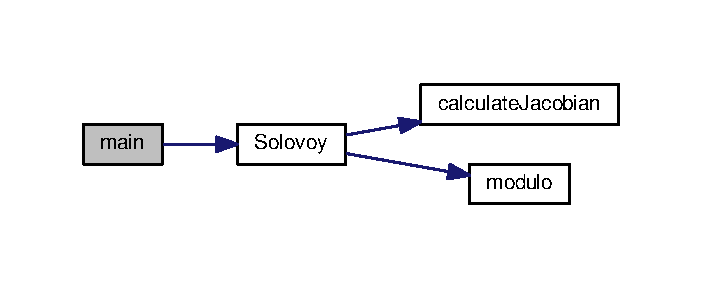
\includegraphics[width=337pt]{Solovay-Strassen_8cpp_ae66f6b31b5ad750f1fe042a706a4e3d4_cgraph}
\end{center}
\end{figure}


\index{Solovay-\/\+Strassen.\+cpp@{Solovay-\/\+Strassen.\+cpp}!modulo@{modulo}}
\index{modulo@{modulo}!Solovay-\/\+Strassen.\+cpp@{Solovay-\/\+Strassen.\+cpp}}
\subsubsection[{\texorpdfstring{modulo(ll base, ll exponent, ll mod)}{modulo(ll base, ll exponent, ll mod)}}]{\setlength{\rightskip}{0pt plus 5cm}{\bf ll} modulo (
\begin{DoxyParamCaption}
\item[{{\bf ll}}]{base, }
\item[{{\bf ll}}]{exponent, }
\item[{{\bf ll}}]{mod}
\end{DoxyParamCaption}
)}\hypertarget{Solovay-Strassen_8cpp_ad815f4d0c344576558f86d0dd549e7f2}{}\label{Solovay-Strassen_8cpp_ad815f4d0c344576558f86d0dd549e7f2}

\begin{DoxyCode}
13 \{
14     \hyperlink{Solovay-Strassen_8cpp_ae1d1ec9482079231e898236e2b23c9ba}{ll} x = 1;
15     \hyperlink{Solovay-Strassen_8cpp_ae1d1ec9482079231e898236e2b23c9ba}{ll} y = base;
16     \textcolor{keywordflow}{while} (exponent > 0)
17     \{
18         \textcolor{keywordflow}{if} (exponent % 2 == 1)
19             x = (x * y) % mod;
20         y = (y * y) % mod;
21         exponent = exponent / 2;
22     \}
23     \textcolor{keywordflow}{return} x % mod;
24 \}
\end{DoxyCode}
\index{Solovay-\/\+Strassen.\+cpp@{Solovay-\/\+Strassen.\+cpp}!Solovoy@{Solovoy}}
\index{Solovoy@{Solovoy}!Solovay-\/\+Strassen.\+cpp@{Solovay-\/\+Strassen.\+cpp}}
\subsubsection[{\texorpdfstring{Solovoy(ll p, int iteration)}{Solovoy(ll p, int iteration)}}]{\setlength{\rightskip}{0pt plus 5cm}bool Solovoy (
\begin{DoxyParamCaption}
\item[{{\bf ll}}]{p, }
\item[{int}]{iteration}
\end{DoxyParamCaption}
)}\hypertarget{Solovay-Strassen_8cpp_a65b69102e0221bb5cfcb7485dffda0d0}{}\label{Solovay-Strassen_8cpp_a65b69102e0221bb5cfcb7485dffda0d0}

\begin{DoxyCode}
73 \{
74     \textcolor{keywordflow}{if} (p < 2) 
75         \textcolor{keywordflow}{return} \textcolor{keyword}{false};
76     \textcolor{keywordflow}{if} (p != 2 && p % 2 == 0) 
77         \textcolor{keywordflow}{return} \textcolor{keyword}{false};
78     \textcolor{keywordflow}{for} (\textcolor{keywordtype}{int} i = 0; i < iteration; i++)
79     \{
80         \hyperlink{Solovay-Strassen_8cpp_ae1d1ec9482079231e898236e2b23c9ba}{ll} a = rand() % (p - 1) + 1;
81         \hyperlink{Solovay-Strassen_8cpp_ae1d1ec9482079231e898236e2b23c9ba}{ll} jacobian = (p + \hyperlink{Solovay-Strassen_8cpp_a8cdb5b6678d3f321ad91e68058ac6306}{calculateJacobian}(a, p)) % p;
82         \hyperlink{Solovay-Strassen_8cpp_ae1d1ec9482079231e898236e2b23c9ba}{ll} mod = \hyperlink{Solovay-Strassen_8cpp_ad815f4d0c344576558f86d0dd549e7f2}{modulo}(a, (p - 1) / 2, p);
83         \textcolor{keywordflow}{if} (!jacobian || mod != jacobian)
84         \{ 
85             \textcolor{keywordflow}{return} \textcolor{keyword}{false};
86         \}
87     \}
88     \textcolor{keywordflow}{return} \textcolor{keyword}{true};
89 \}
\end{DoxyCode}


Here is the call graph for this function\+:
\nopagebreak
\begin{figure}[H]
\begin{center}
\leavevmode
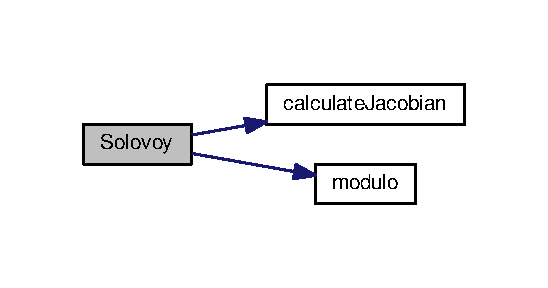
\includegraphics[width=263pt]{Solovay-Strassen_8cpp_a65b69102e0221bb5cfcb7485dffda0d0_cgraph}
\end{center}
\end{figure}



%--- End generated contents ---

% Index
\backmatter
\newpage
\phantomsection
\clearemptydoublepage
\addcontentsline{toc}{chapter}{Index}
\printindex

\end{document}
